\documentclass[aspectratio=169,xcolor=dvipsnames, t]{beamer}

\usepackage{cp24}
\usepackage[square,numbers]{natbib}

\bibliographystyle{ACM-Reference-Format}

%*************************************************************************************************************
\title[Customizable Roundtrips with Tour4Me]{Customizable Roundtrips with Tour4Me}
\subtitle{Meta-heuristic Approaches for Personalized Running and Cycling Routes}
\author[Lisa Salewsky]{
	Lisa Salewsky
}


\institute[TU Dortmund]{
	\begin{minipage}[t][2.3cm][b]{0.7\textwidth}
		\centering
		\begin{tikzpicture}[remember picture,overlay]
			\node[inner sep=0] at (2.5,-0.8) {
\includegraphics[scale=0.1]{logo.png}};
		\end{tikzpicture}
		TU Dortmund, Fakultät für Informatik\\
		\vspace{1.5cm}
		Reviewer:\\
		Prof. Dr. Kevin Buchin\\
		Mart Hagedoorn, M. Sc.
	\end{minipage}
	
}
\date[April 25th, 2024]{April 25th, 2024}
\beamertemplatenavigationsymbolsempty %Navigantionszeite unten aus
%*************************************************************************************************************
%\usetheme{Malmoe} 
%\usetheme{Madrid}
%\usecolortheme{rose} %schwache farben
% Themes:
%AnnArbor | Antibes | Bergen |Berkeley | Berlin | Boadilla |boxes | CambridgeUS | Copenhagen |Darmstadt | default | Dresden |
%Frankfurt | Goettingen |Hannover | Ilmenau | JuanLesPins | Luebeck | Madrid | Malmoe | Marburg |
%Montpellier | PaloAlto | Pittsburgh |Rochester | Singapore | Szeged |Warsaw
\useinnertheme{rounded}
%\useoutertheme{shadow} %schattierung in den Rechtecken der Blocken -- nix
%*************************************************************************************************************


% Customize the table of contents
\setbeamertemplate{section in toc}[square]
\setbeamertemplate{subsection in toc}[square]
\setbeamertemplate{section/subsection in toc}[square]
\setbeamercolor{section number projected}{bg=tu_green_full,fg=white}
\setbeamercolor{subsection number projected}{bg=tu_green_full,fg=white}

% Customize all the bulletpoints
\setbeamertemplate{items}[square]

% Customize the link colors
\hypersetup{
	colorlinks=true,
	linkcolor=tu_green_full2,
	urlcolor=tu_green_full2,
	citecolor=tu_green_full2
}

\setbeamercolor{block title}{bg=tu_light_green_full2, fg=black}
\setbeamercolor{block body}{bg=tu_light_green_full3, fg=black}


\begin{document}
	%*************************************************************
	\begin{frame}
		\thispagestyle{empty}
		\titlepage
	\end{frame}
	%*************************************************************
%	
%	\begin{frame}{Agenda}
%		\centering	
%		\tableofcontents
%	\end{frame}
	
	\section{Introcuction}
	
	\begin{frame}{Introcuction}
		\vspace{0.25cm}
		Why do we need an app for creating round trips?
		\only<2>{	
			\begin{figure}
				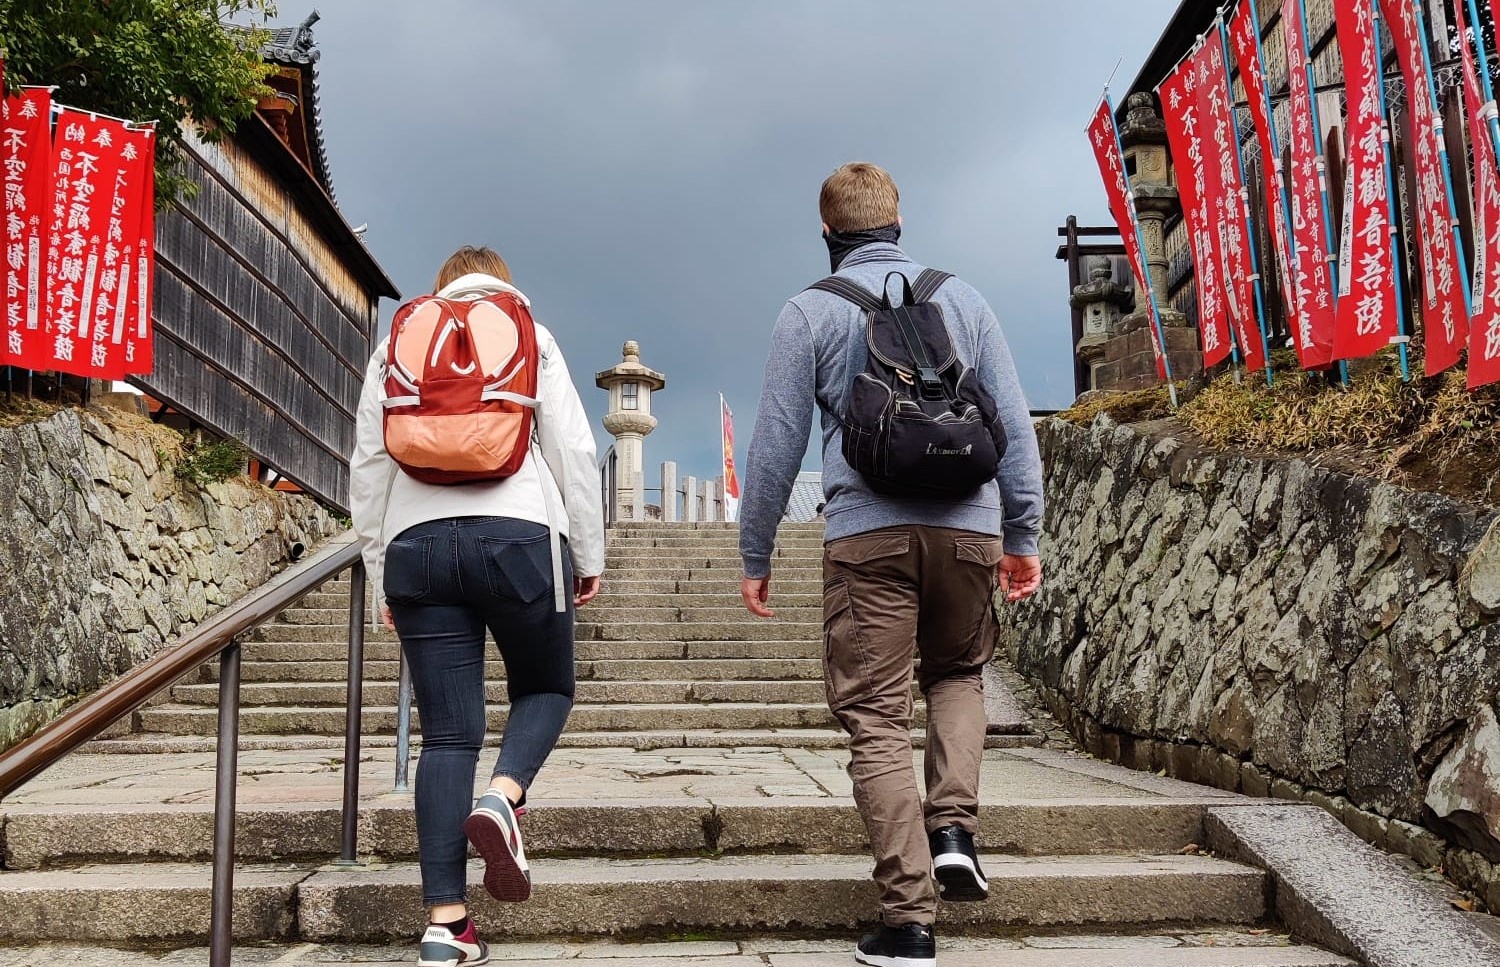
\includegraphics[height=0.6\textheight]{images/IMG-20231124-WA0010-cropped.jpg}
			\end{figure}}
		\only<3>{	
			\begin{figure}
				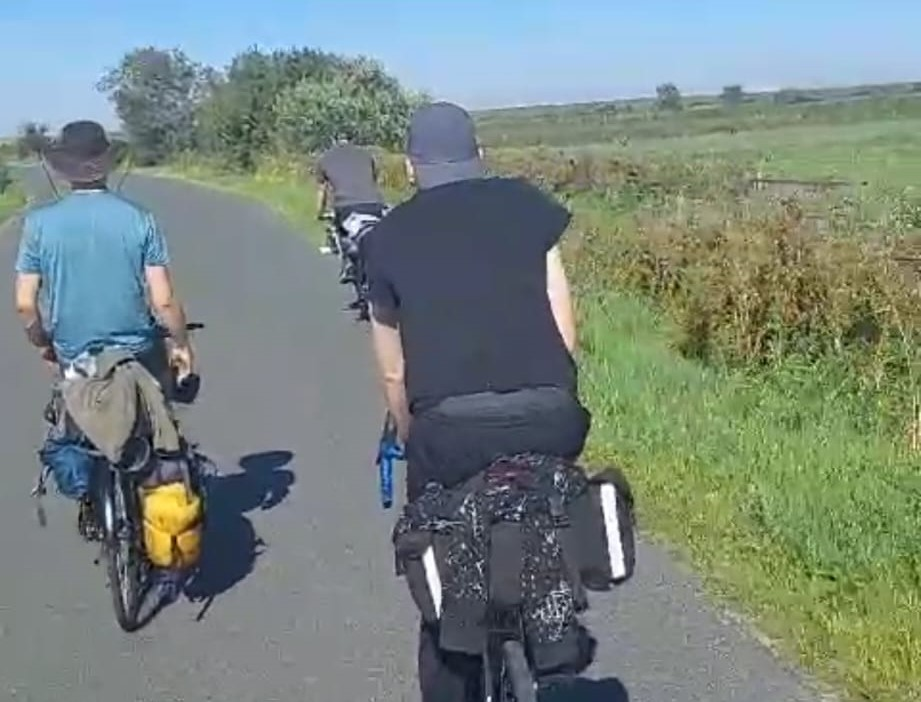
\includegraphics[height=0.6\textheight]{images/IMG-20231124-WA0039-cropped.jpg}
			\end{figure}}
		\only<4>{	
			\begin{figure}
				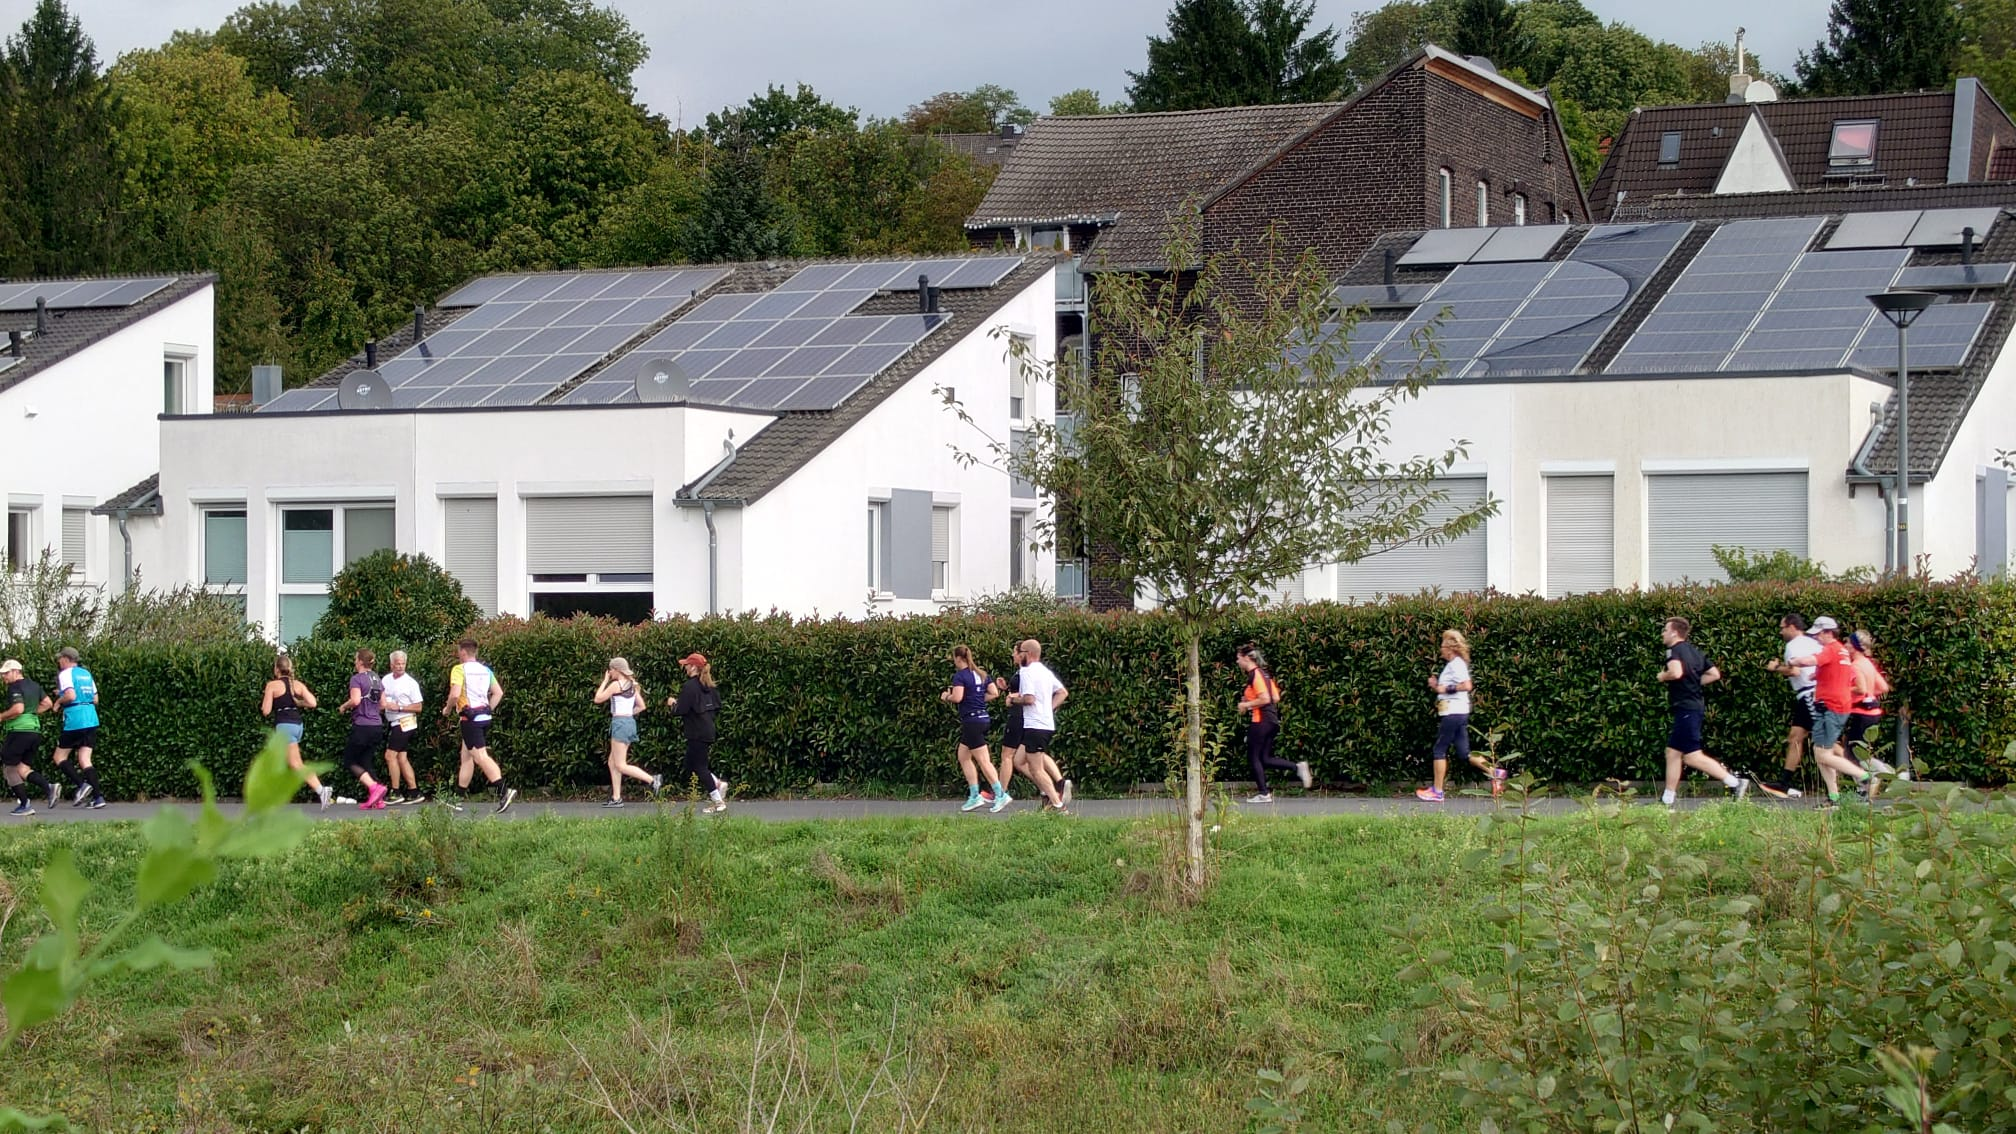
\includegraphics[height=0.6\textheight]{images/WhatsApp Bild 2023-11-24 um 14.35.53_5752c78a.jpg}
			\end{figure}}
	\end{frame}
	\begin{frame}{Introcuction}
		\vspace{0.25cm}
		Why do we need an app for creating round trips?
		\begin{columns}
			\begin{column}{0.48\textwidth}
				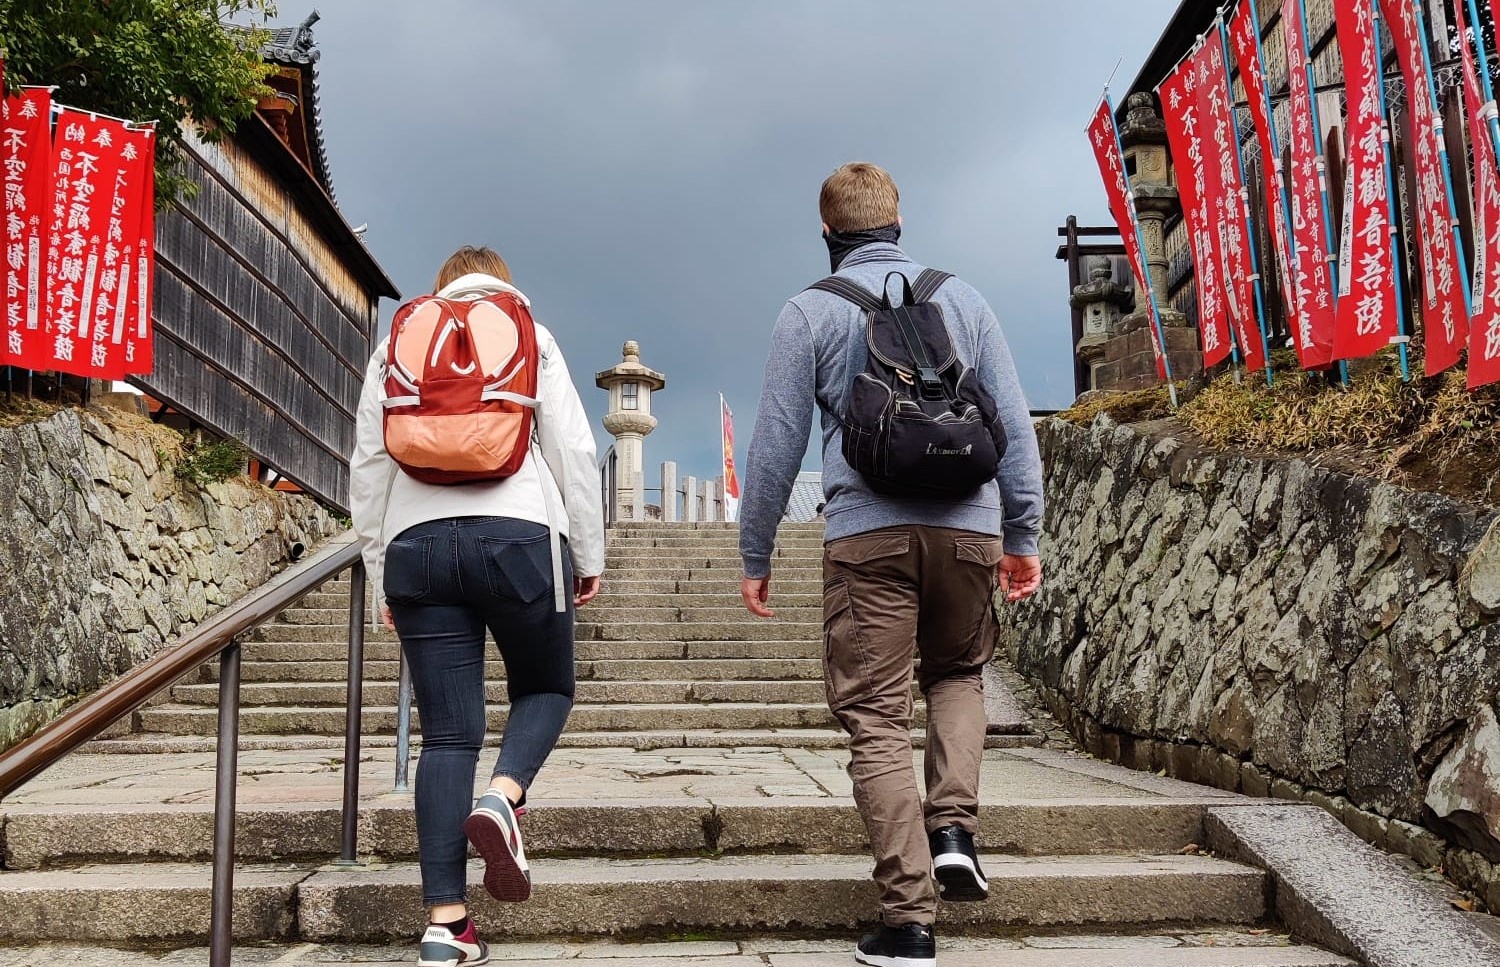
\includegraphics[height=0.3\textheight]{images/IMG-20231124-WA0010-cropped.jpg}
			\vspace{-1.5cm}
				\begin{flushright}
					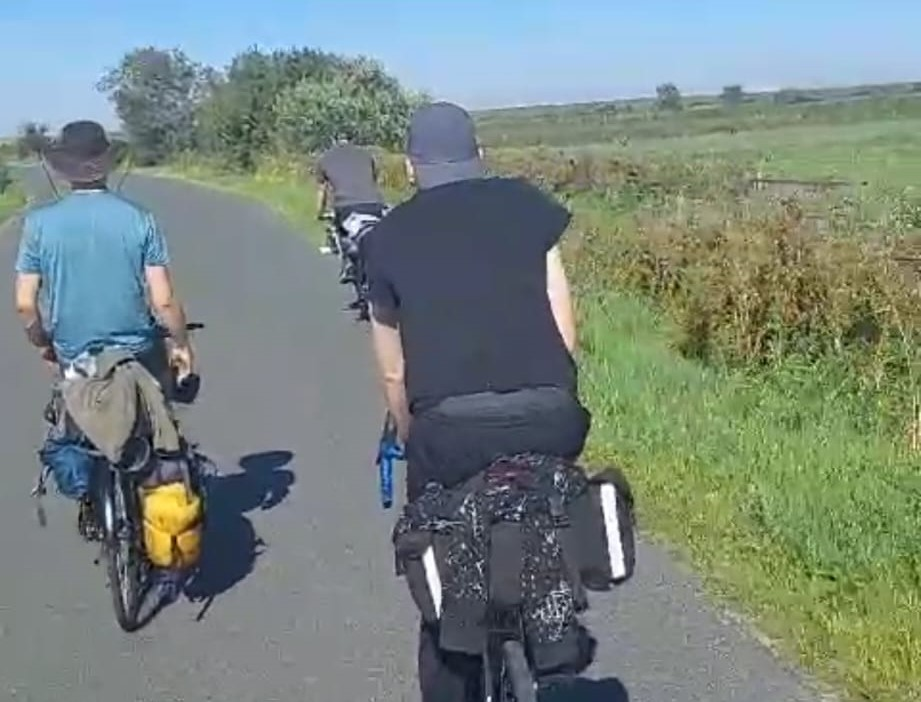
\includegraphics[height=0.3\textheight]{images/IMG-20231124-WA0039-cropped.jpg}
				\end{flushright}
			\vspace{-1cm}
				\begin{flushleft}
					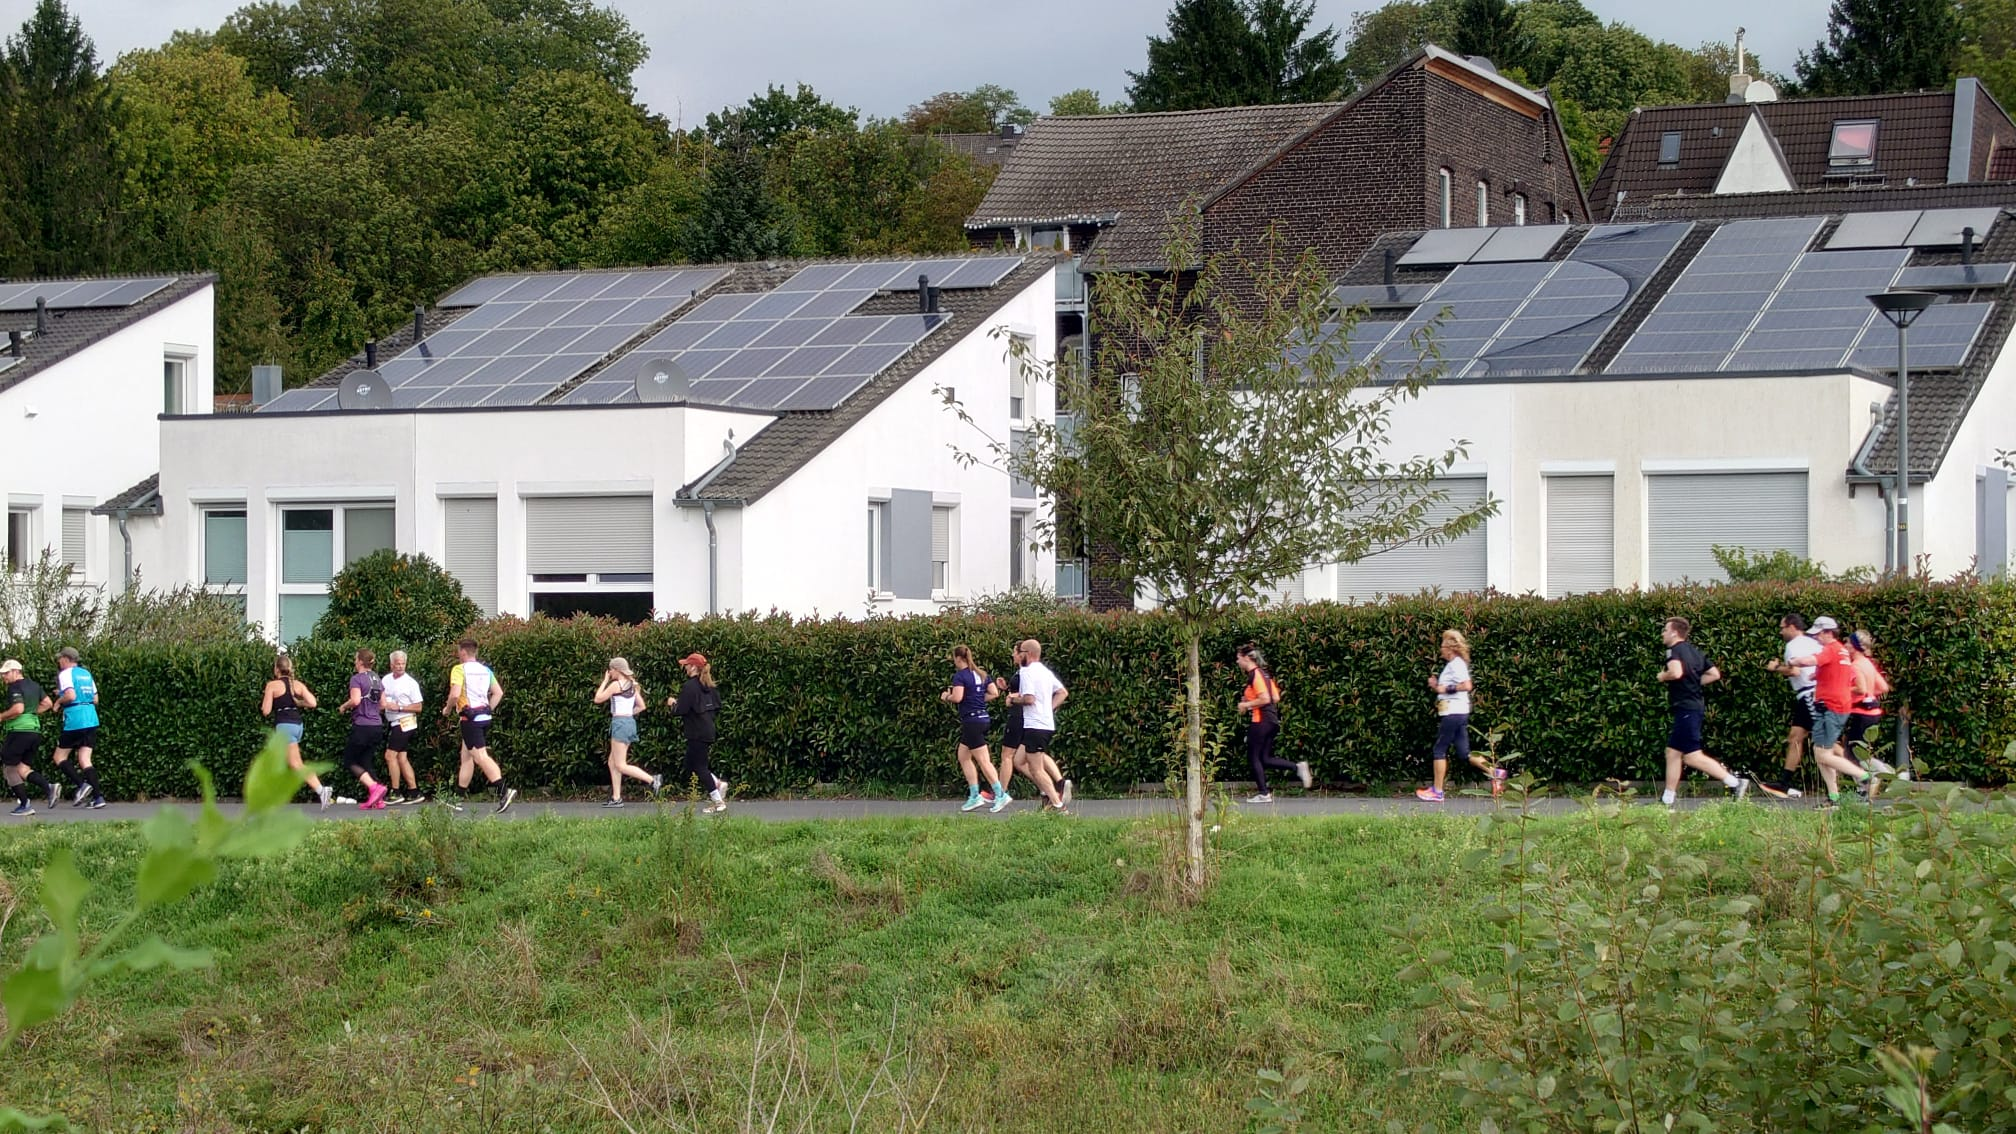
\includegraphics[height=0.3\textheight]{images/WhatsApp Bild 2023-11-24 um 14.35.53_5752c78a.jpg}
				\end{flushleft}
		\end{column}
		\begin{column}{0.48\textwidth}
			\vspace{-2.5cm}
			\begin{block}{Similarities}
				\pause
				\begin{itemize}
					\only<2>{\item Trips from A to B}
					\only<3->{\item Trips from A to B?}
					\item<4-> Oftentimes round trips when done as pastime hobbies
					\item<5-> Want for tours that can be personalized according to subjective criteria
				\end{itemize}
			\end{block}	
			\begin{itemize}	
			\item<6-> Many existing ideas for shortest paths from A to B
				\only<7>{\item Not many approaches to calculate round trips}
				\only<8->{\item Not many approaches to calculate round trips with preferences}
			\end{itemize}
		\end{column}
		\end{columns} ~\\		
	\end{frame}
	
%	\begin{frame}{Einleitung}
%	\vspace{0.25cm}
%	Warum eine App zum Erstellen von Rundrips?
%	\begin{itemize}	
%		\item<1-> Viele Lösungen für kürzeste Wege von A nach B
%		\item<2-> Optimieren alltägliche Routen
%		\item<3-> Joggen und Radfahren in der Freizeit:
%		\begin{itemize}	
%		\item<3-> Weitere Bedingungen für gute Strecken nötig
%		\only<4>{\item Und kaum Ansätze für Rundtrips}
%		\only<5->{\item Und kaum Ansätze für Rundtrips mit Präferenzen}
%		\end{itemize}
%	\end{itemize}
%	\end{frame}

	\begin{frame}{Introcuction}
		\vspace{0.25cm}
		What is an appealing tour?\\
		\pause
		\vspace{-0.2cm}
		\begin{minipage}[t]{0.48\textwidth}
			\begin{itemize}[<+->]
				\item Very subjective and based on individual preferences
				\item Many different potential factors
				\begin{itemize}[<+->]
					\item Path type (street, path (in the forest), cycling path etc.)
					\item Ground (tar, gravel, sand, soil, etc.)
					\item Slope
					\item Surroundings (forest, park, residential area, etc.)
					\item Shape (round, U-Turn, complex with many turns, etc.)
				\end{itemize}
				\item Influence of these on the tour quality is very subjective 
		\end{itemize}
		\end{minipage}
		\begin{minipage}[t][0.7\textheight][b]{0.48\textwidth}
			\only<4>{
				\includegraphics[height=0.5\textheight]{images/IMG_20220921_181918.jpg}
				\vspace{-4cm}
				\begin{flushright}
					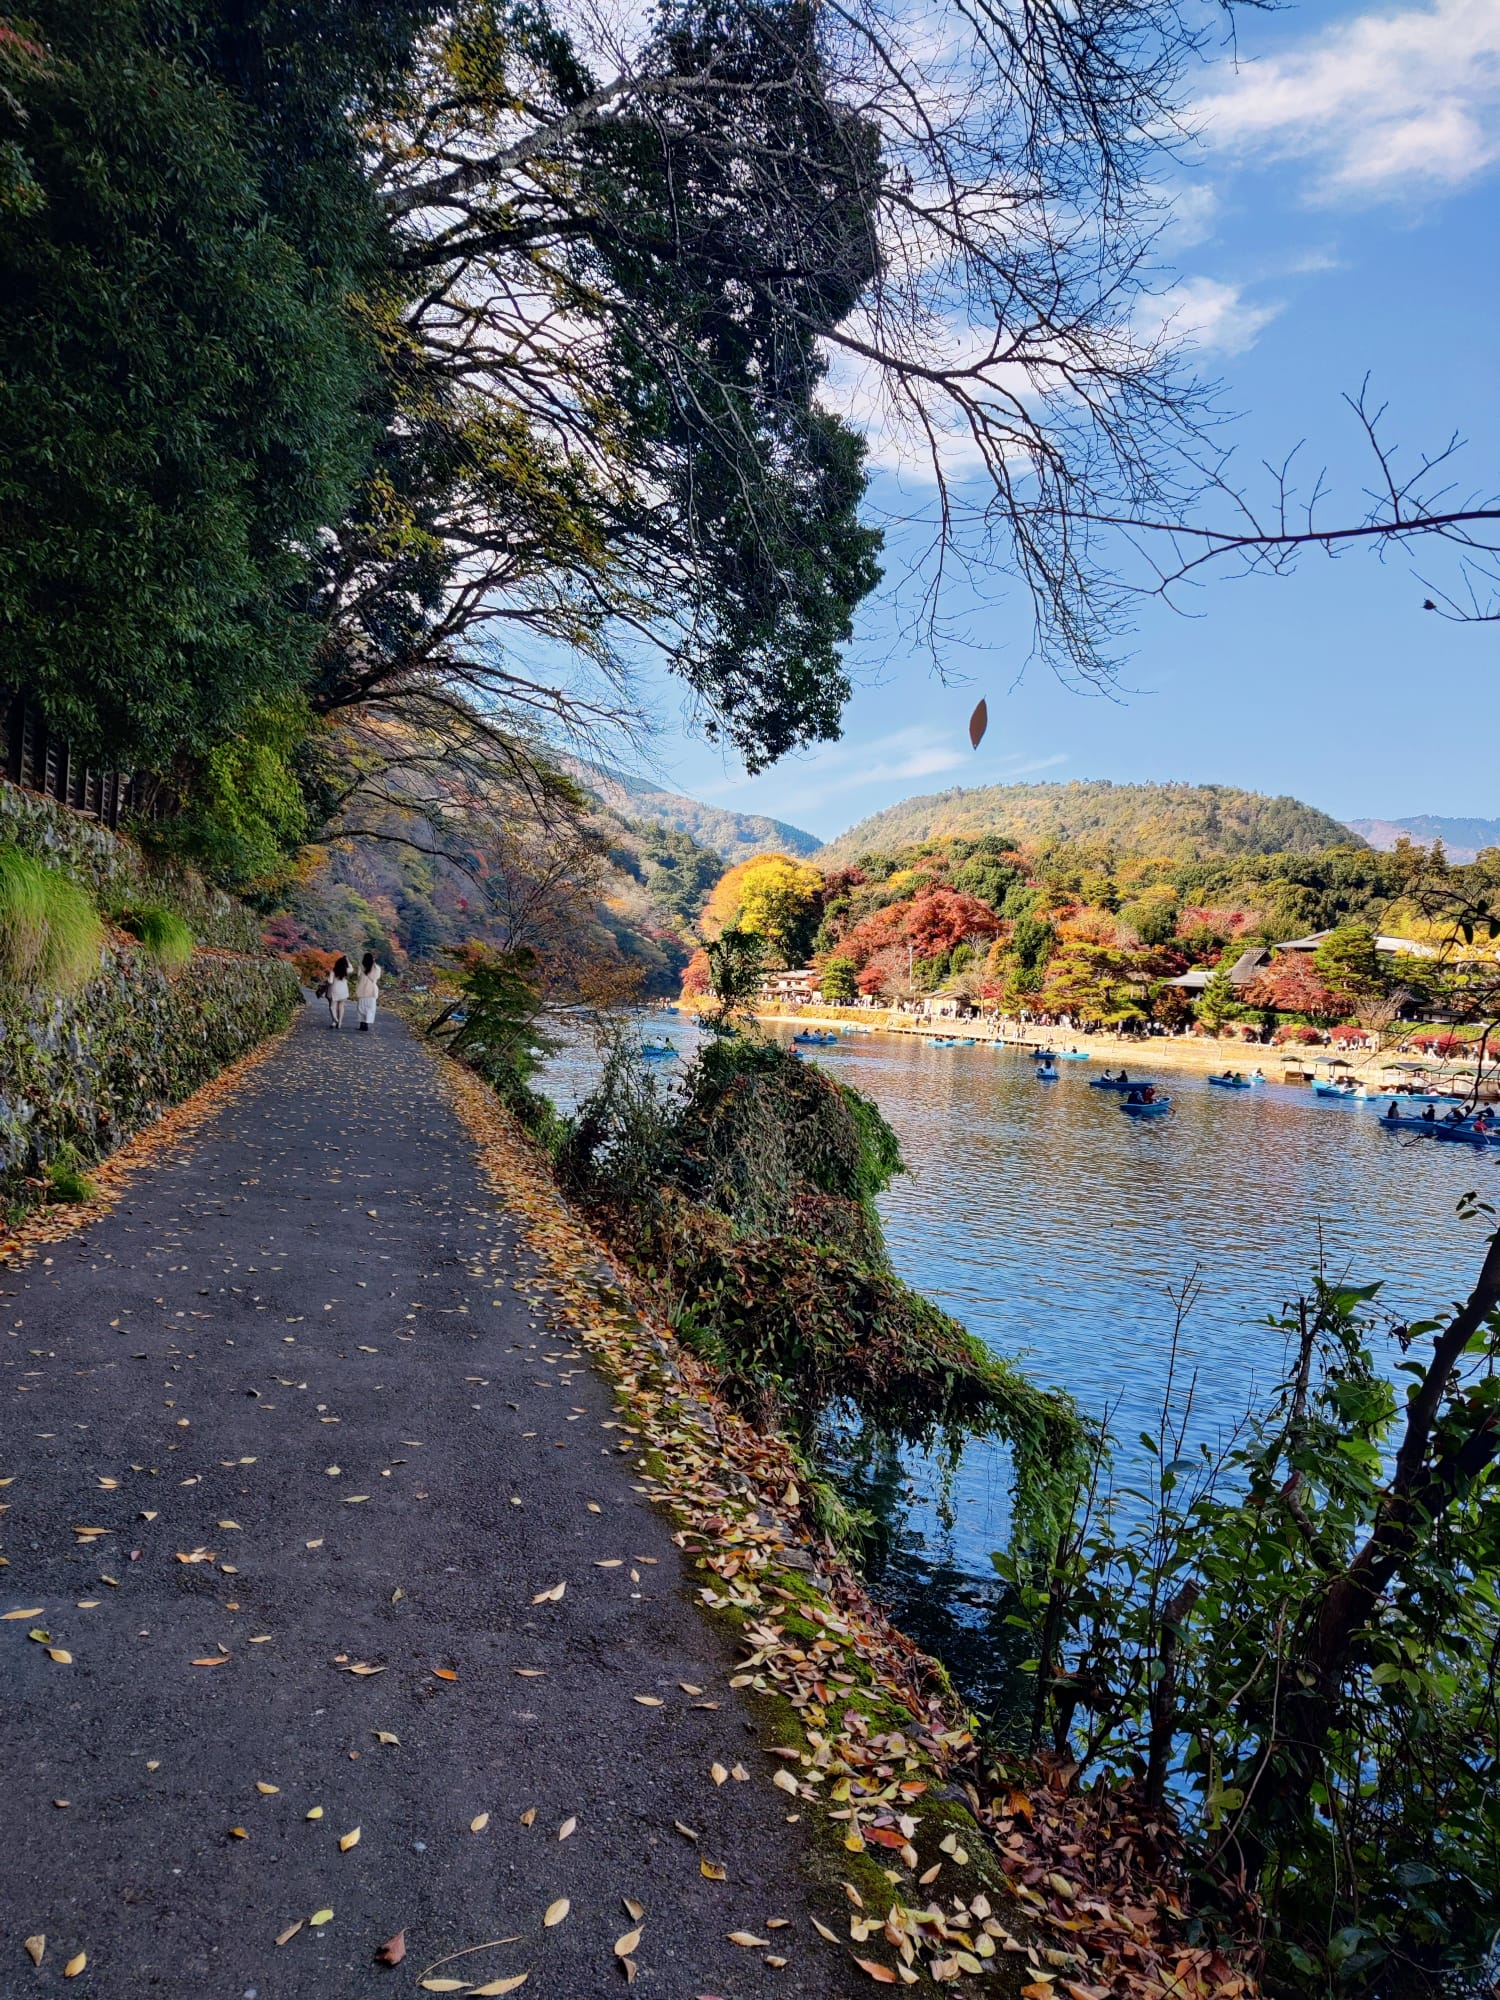
\includegraphics[height=0.5\textheight]{images/IMG-20231124-WA0038.jpg}
				\end{flushright}
				\vspace{-1cm}
				\begin{flushleft}
					\includegraphics[height=0.3\textheight]{images/DSC00708.JPG}
				\end{flushleft}}
			\only<5>{
				\includegraphics[height=0.3\textheight]{images/DSC08658.JPG}
				\vspace{-2cm}
				\begin{flushright}
					\includegraphics[height=0.5\textheight]{images/IMG_20220921_181918.jpg}
				\end{flushright}
				\vspace{-2cm}
				\begin{flushleft}
					\includegraphics[height=0.3\textheight]{images/DSC03182.JPG}
				\end{flushleft}}
			\only<6>{
				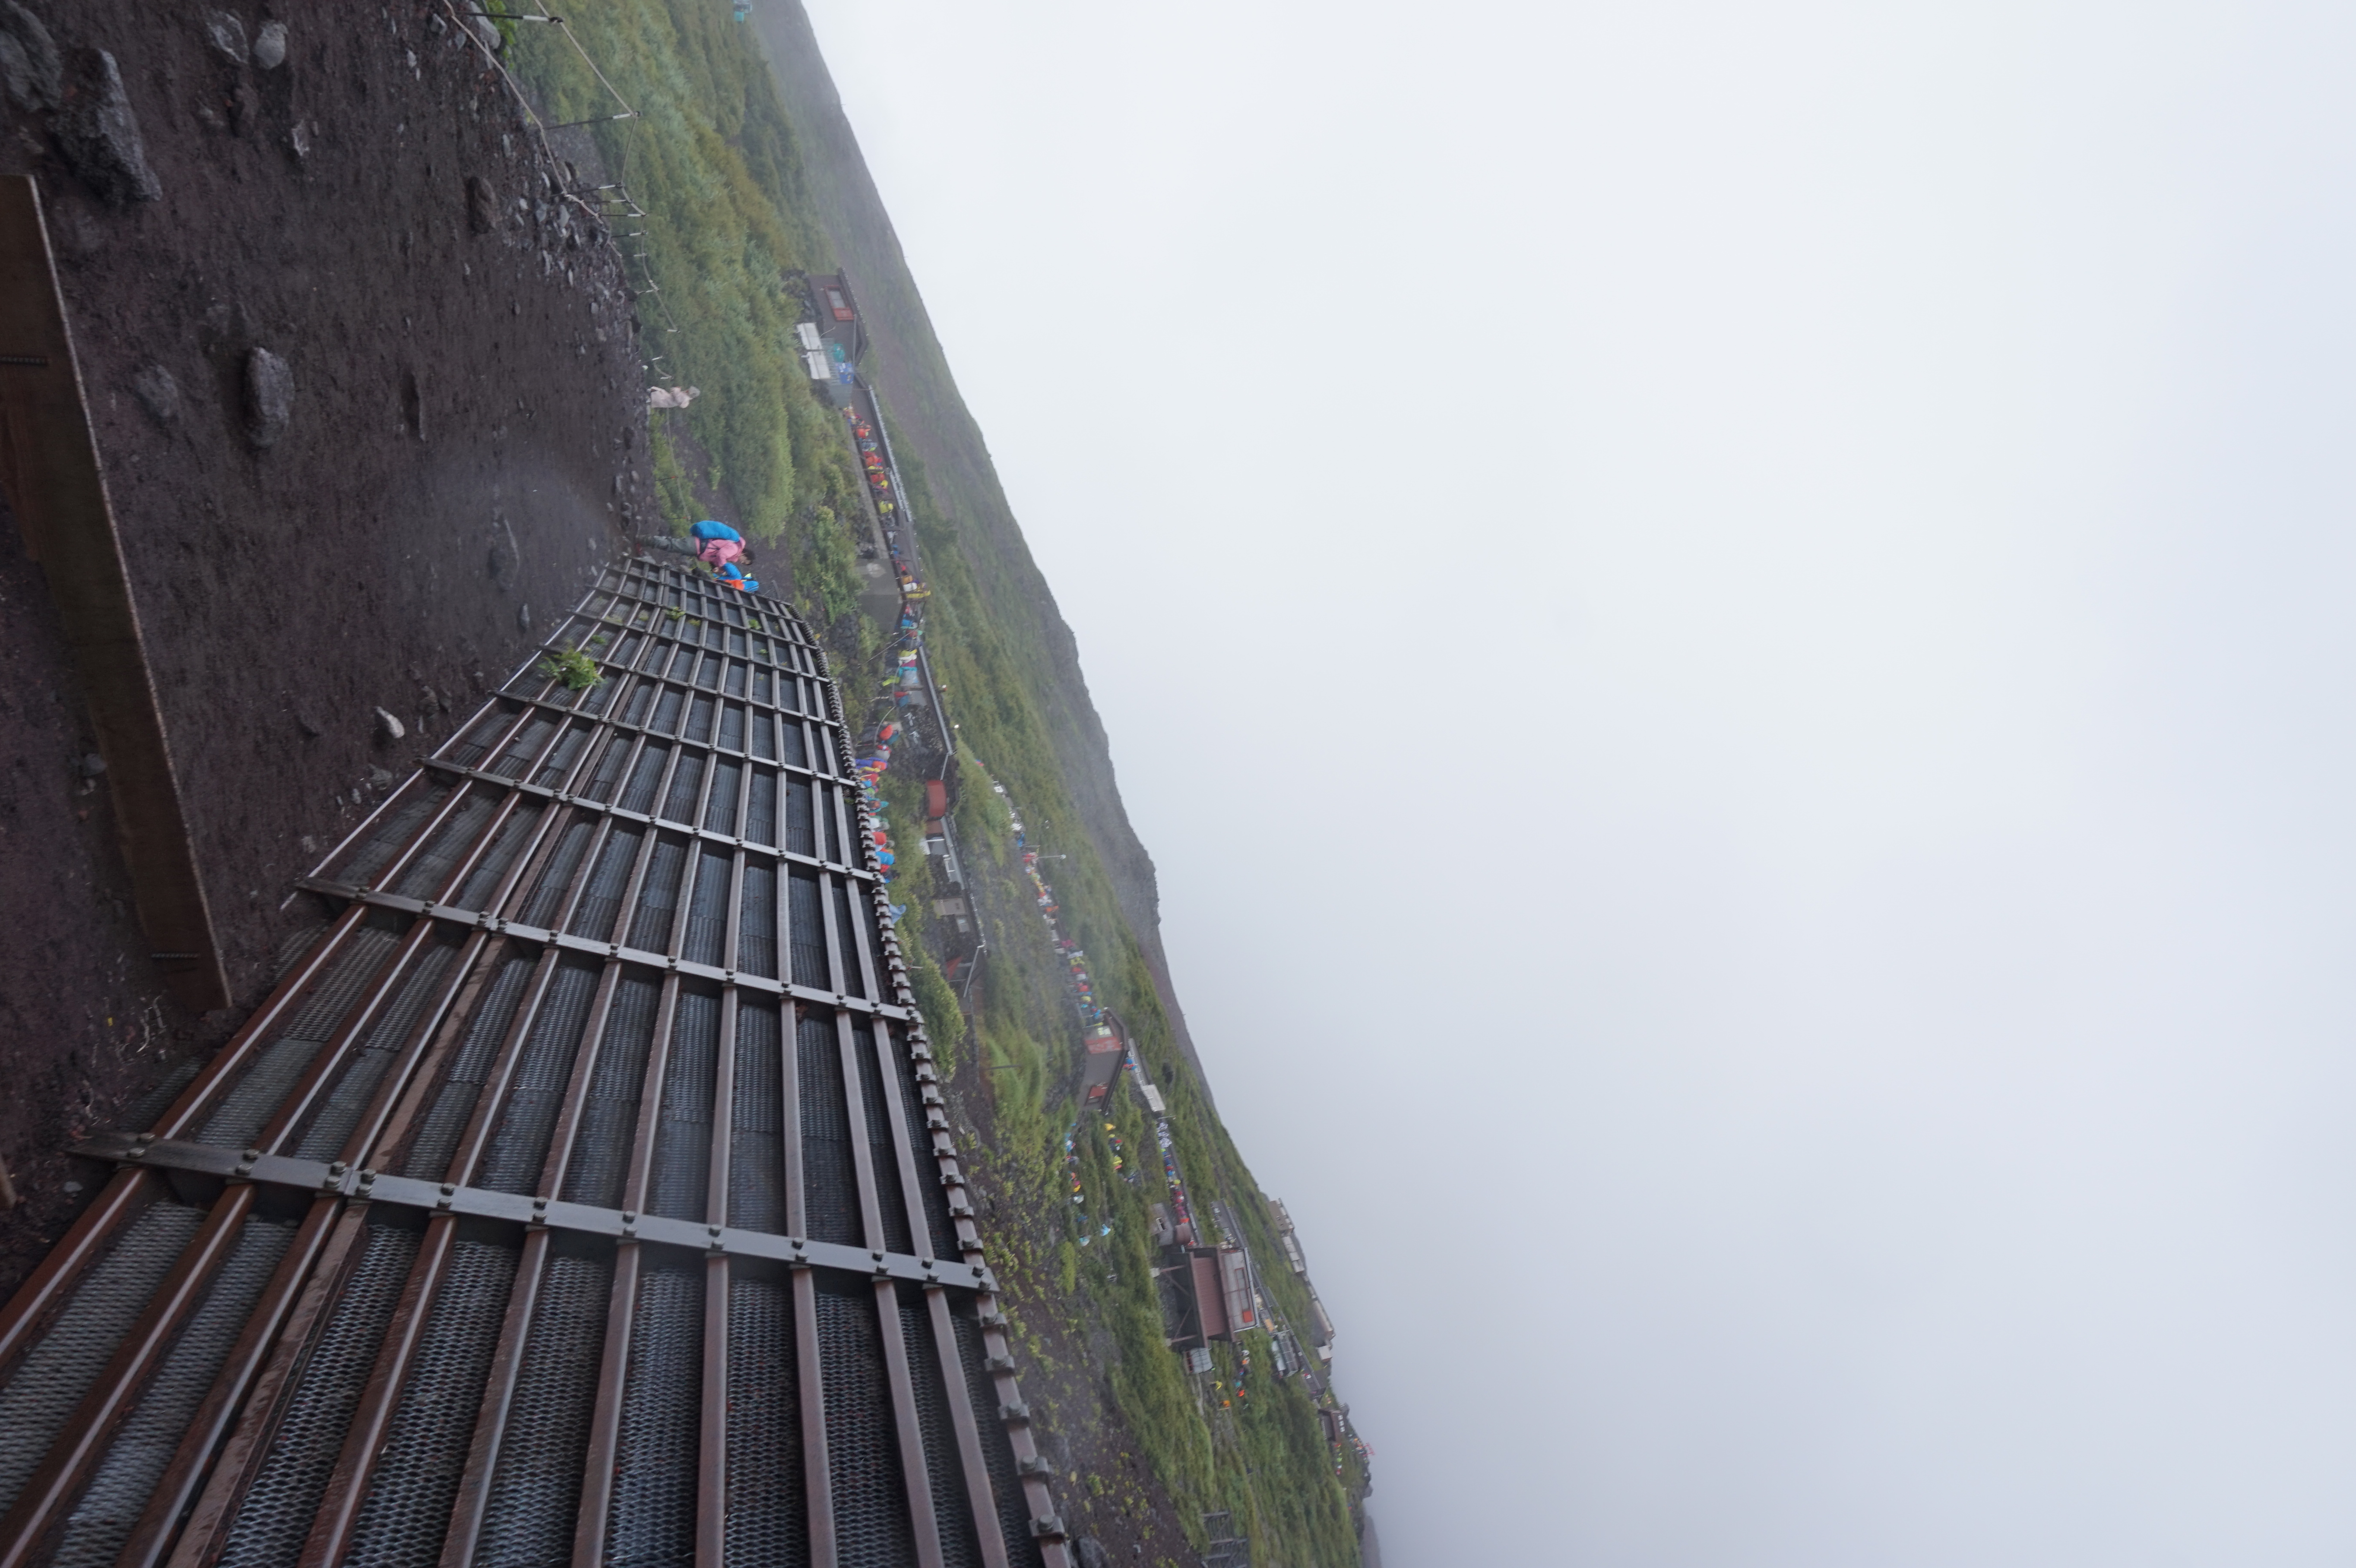
\includegraphics[height=0.3\textheight, angle=90]{images/DSC00758.JPG}
				\vspace{-3cm}
				\begin{flushright}
					\includegraphics[height=0.3\textheight]{images/DSC08658.JPG}
				\end{flushright}
%				\vspace{0.5cm}
				\begin{flushleft}
					\includegraphics[height=0.3\textheight]{images/DSC03182.JPG}
				\end{flushleft}}
			\only<7>{
				\includegraphics[height=0.3\textheight]{images/DSC03653.JPG}
				\vspace{-3cm}
				\begin{flushright}
					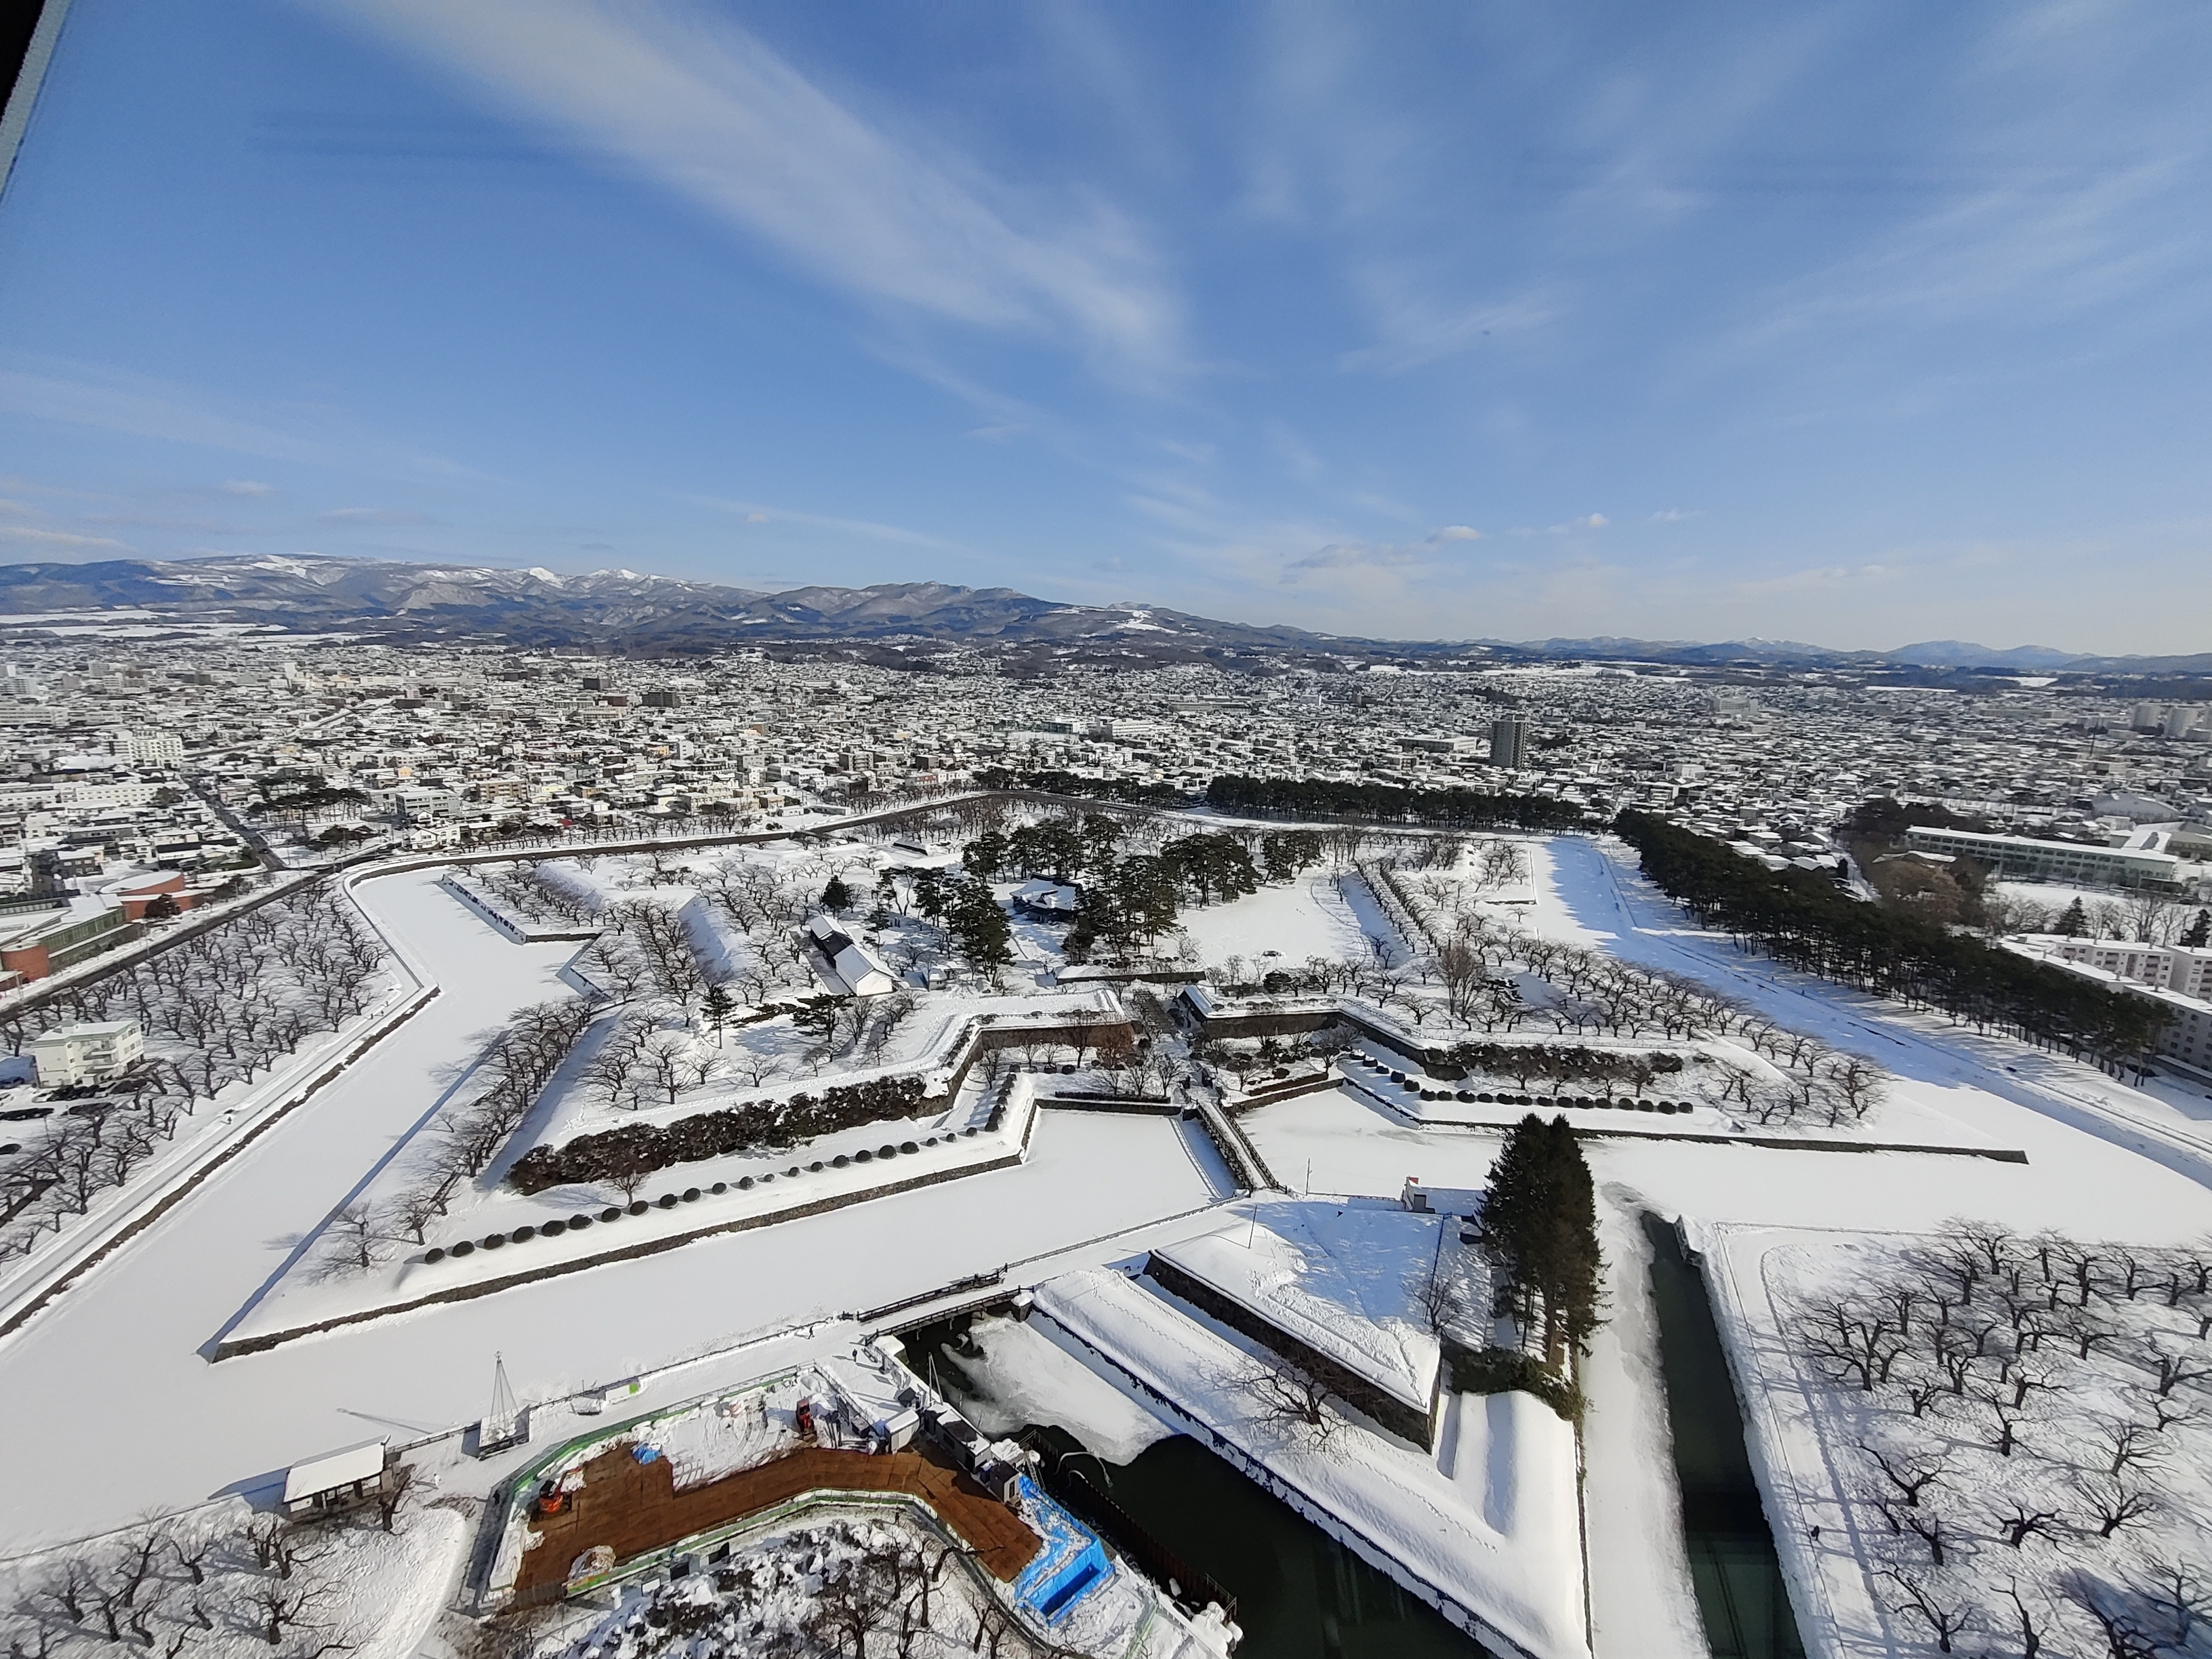
\includegraphics[height=0.3\textheight]{images/IMG_20230208_095155.jpg}
				\end{flushright}
				\vspace{0.5cm}
				\begin{flushleft}
					\includegraphics[height=0.3\textheight]{images/IMG_20221008_161529.jpg}
				\end{flushleft}
				\vspace{-3cm}
				\begin{flushright}
					\includegraphics[height=0.3\textheight]{images/IMG_20220913_171859.jpg}
				\end{flushright}}
			\only<8>{
			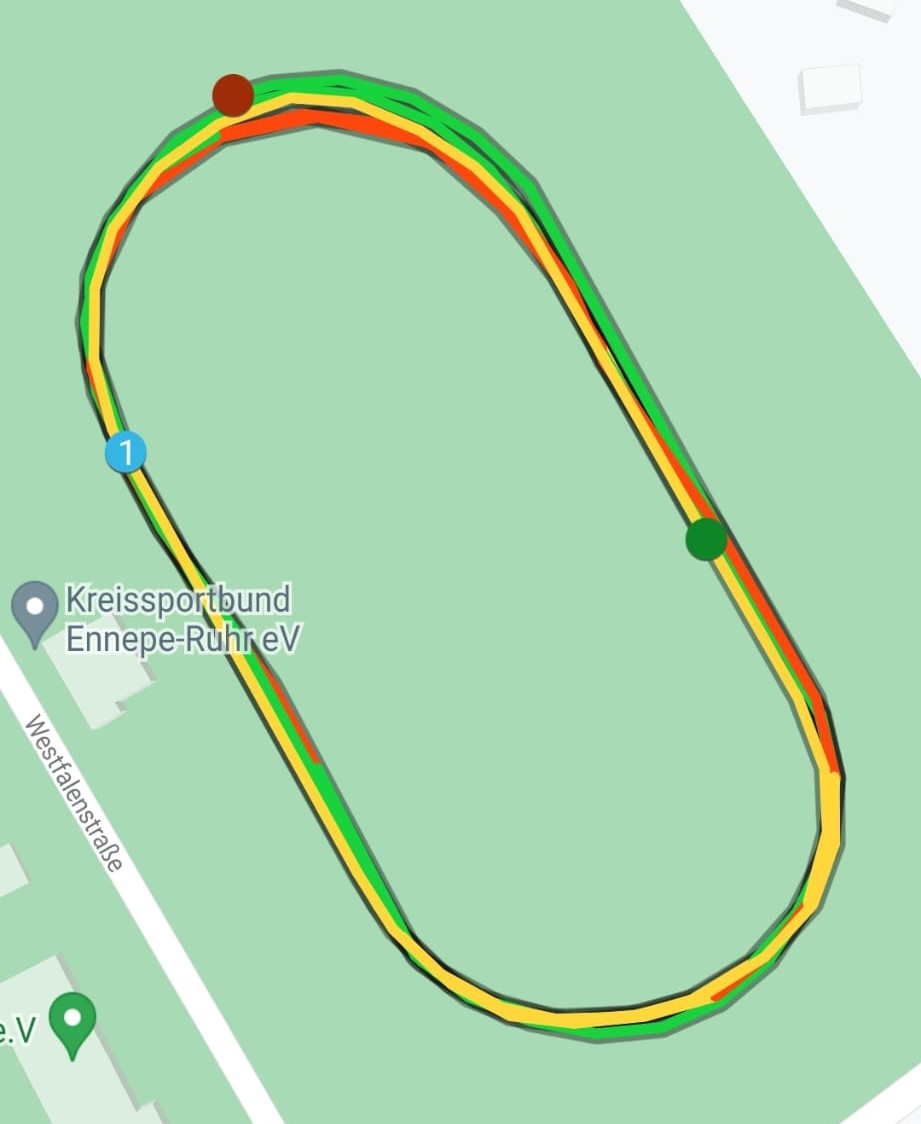
\includegraphics[height=0.4\textheight]{images/laufstrecke_rund.jpg}
			\vspace{-3cm}
				\begin{flushright}
					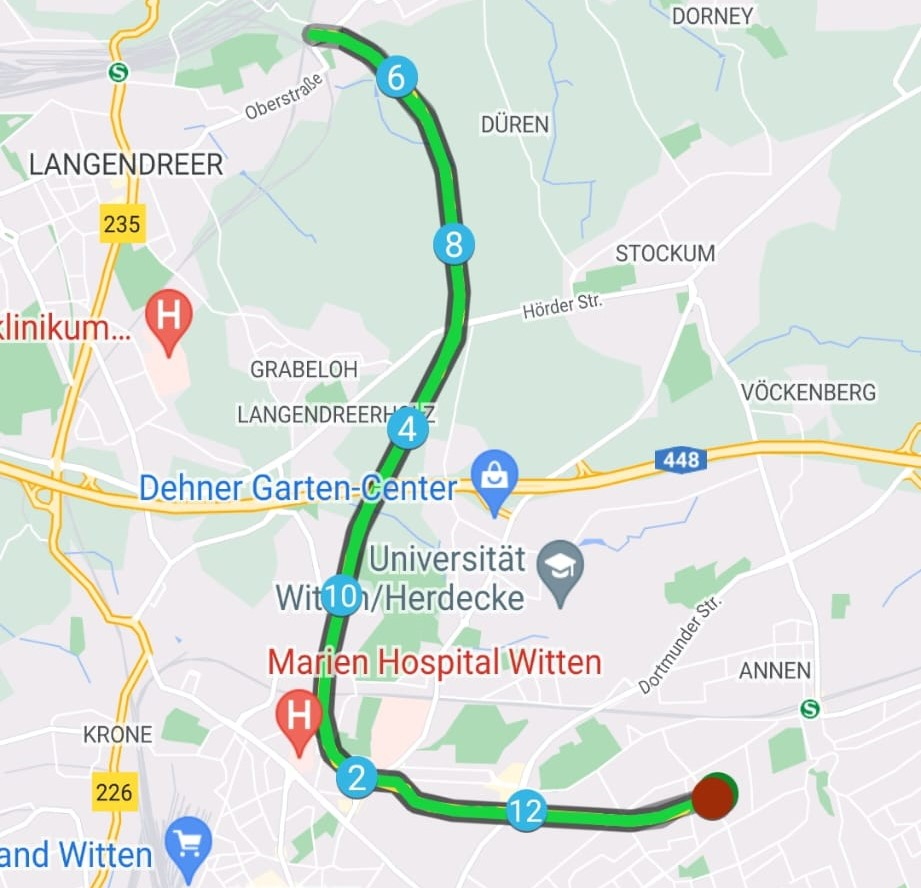
\includegraphics[height=0.4\textheight]{images/laufstecke_uturn.jpg}
				\end{flushright}
				%				\vspace{0.5cm}
				\begin{flushleft}
					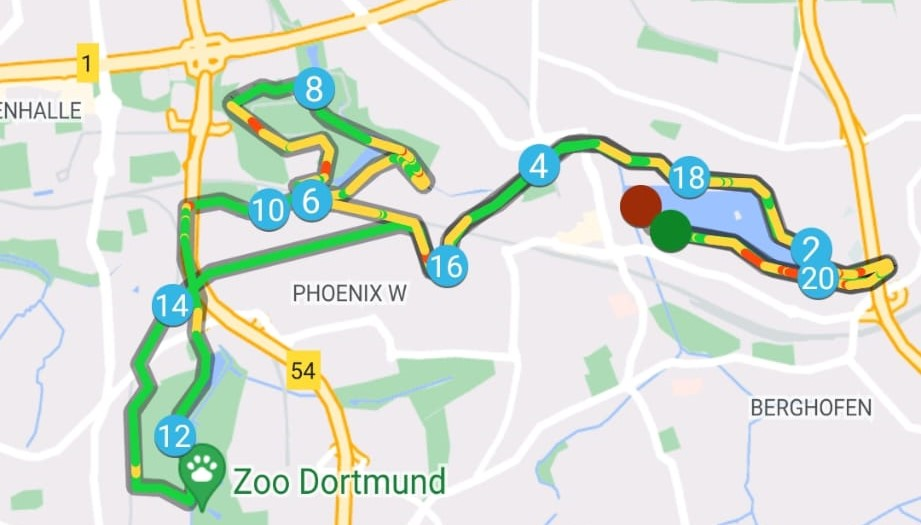
\includegraphics[height=0.3\textheight]{images/laufstrecke_komplex.jpg}
				\end{flushleft}}
		\end{minipage}
 	\end{frame}
	
	\begin{frame}{Tour4Me}
		\vspace{0.25cm}
	\centering	
	\only<1>{\includegraphics[height=0.8\textheight]{images/tour4me_full.png}}
	\only<2>{\includegraphics[height=0.8\textheight]{images/tour4me_settings.png}}
	\only<3>{\includegraphics[height=0.8\textheight]{images/tour4me_mincost_example.png}}
	\only<4>{\includegraphics[height=0.8\textheight]{images/tour4me_route_information.png}}
	
	\end{frame}
	
	\section{Goal}
	\begin{frame}
		\vspace{0.25cm}
		What are the goals? What did I do so far?
		\pause
		\begin{itemize}[<+->]
			\item Basis: Tour4Me
			\item Add extensions and improve general usability of the app
		\end{itemize}
		\uncover<3->{
			\begin{minipage}[t][3.7cm][b]{0.48\linewidth}
				\only<4-13>{
				\begin{block}{ Algorithmic extensions: meta heuristics}	
					\pause	
					\only<4-8>{
					\begin{itemize}[<+->]
						\item AntColony
						\item Simulated Annealing
						\item Genetic
						\item Combinations
					\end{itemize}
					}		
					\only<9>{
					\begin{itemize}
						\item AntColony \textbigcircle
						\item Simulated Annealing
						\item Genetic
						\item Combinations
					\end{itemize}
					}	
					\only<10>{
					\begin{itemize}
						\item AntColony \textbigcircle
						\item Simulated Annealing \textbigcircle
						\item Genetic
						\item Combinations
					\end{itemize}
					}	
					\only<11-13>{
					\begin{itemize}
						\item AntColony \textbigcircle
						\item Simulated Annealing \textbigcircle
						\item Genetic
						\item Combinations \textbigcircle
					\end{itemize}
					}
				\end{block}}
			\only<4-13>{\textcolor{white}{a}}
			\only<14>{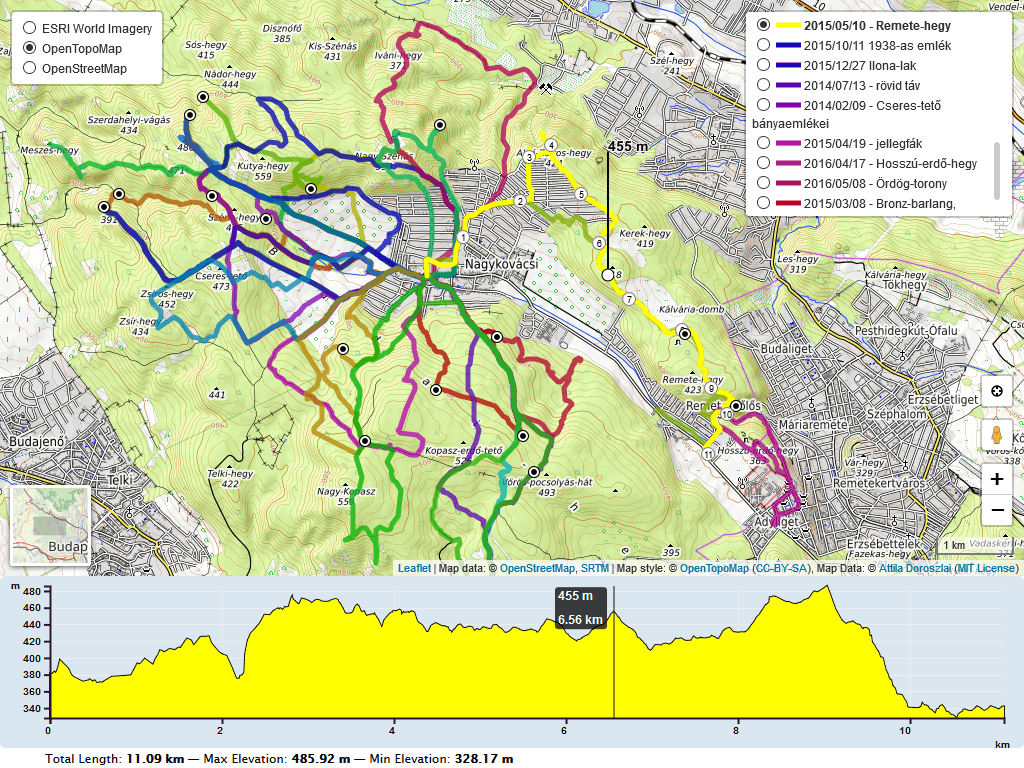
\includegraphics[height=0.5\textheight]{images/GUIIllustration.png}\footnote[frame]{https://github.com/Raruto/leaflet-elevation}}
			\only<15>{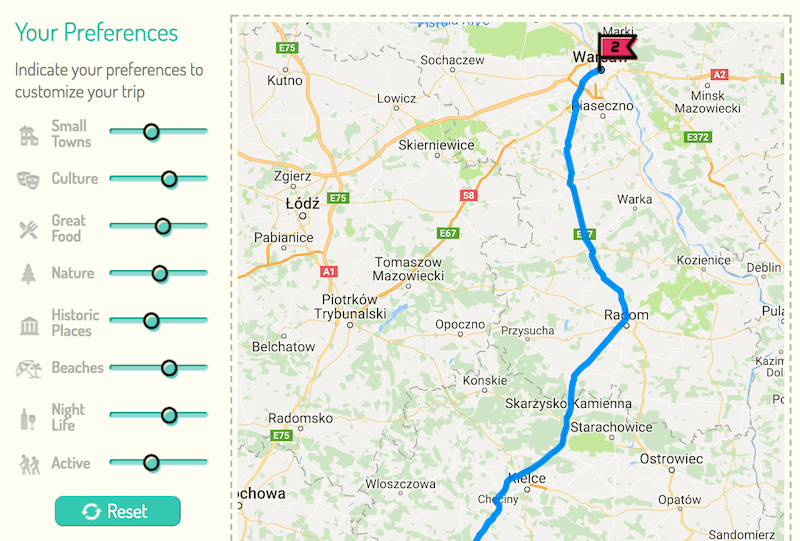
\includegraphics[height=0.5\textheight]{images/GUISliderIlustration.png}\footnote[frame]{https://www.smashingmagazine.com/2017/07/designing-perfect-slider/}}
			\only<16->{
				\begin{block}{ Algorithmic extensions: meta heuristics}		
					\begin{itemize}
						\item AntColony \textbigcircle
						\item Simulated Annealing \textbigcircle
						\item Genetic
						\item Combinations \textbigcircle
					\end{itemize}
			\end{block}
			\textcolor{white}{a}}
			\end{minipage}
			\hfill
			\begin{minipage}[t][4.1cm][b]{0.48\linewidth}
				\only<5>{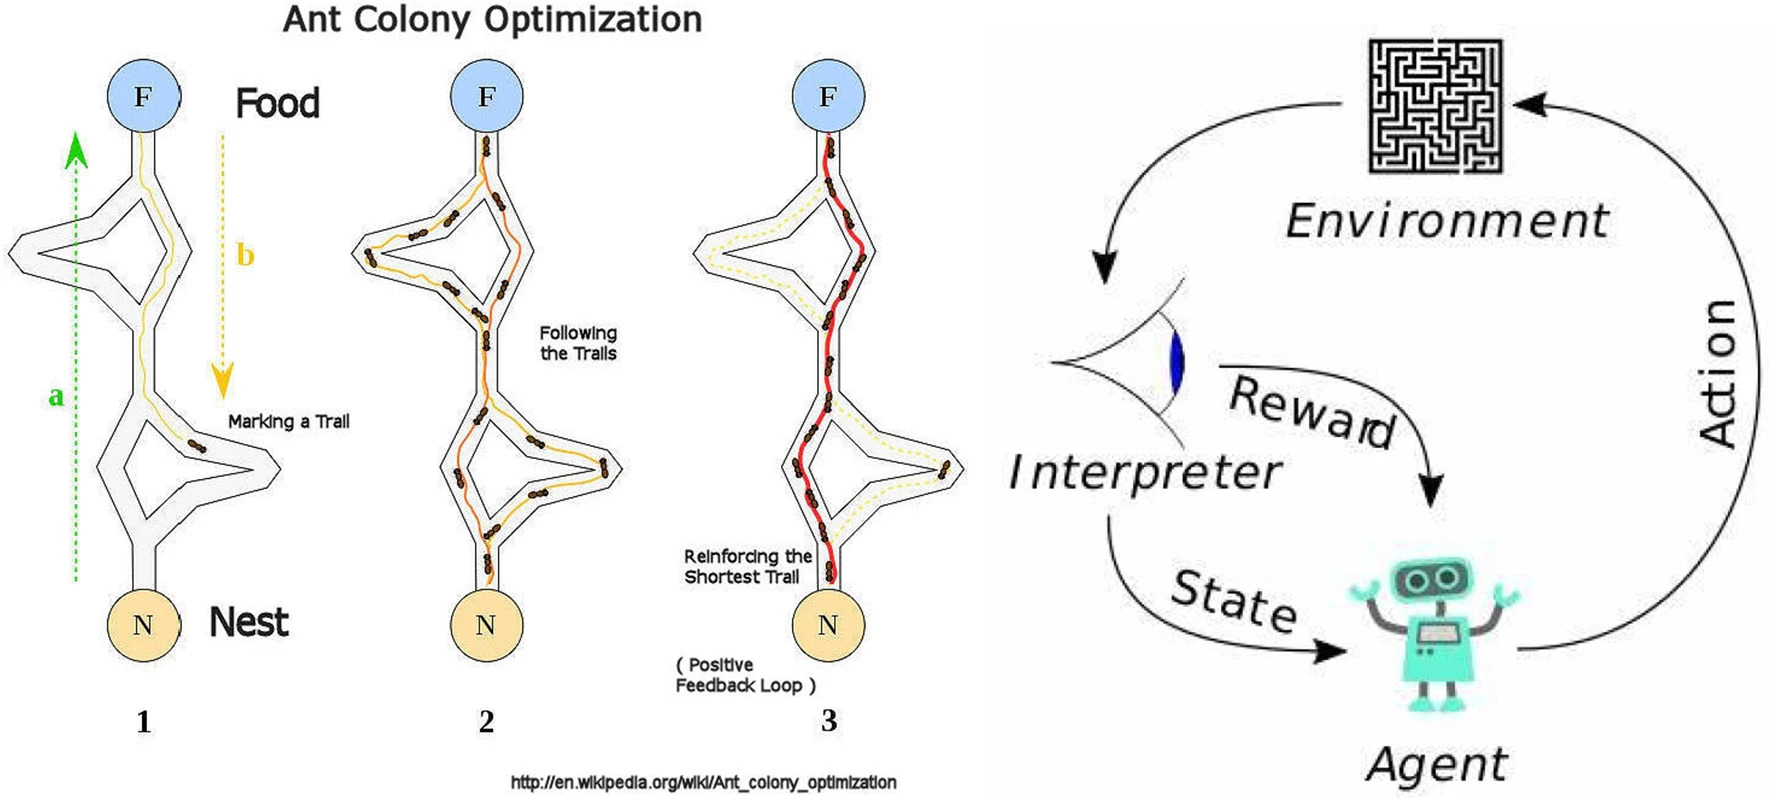
\includegraphics[height=0.5\textheight]{images/antColonyIllustration.png}}
				\only<6>{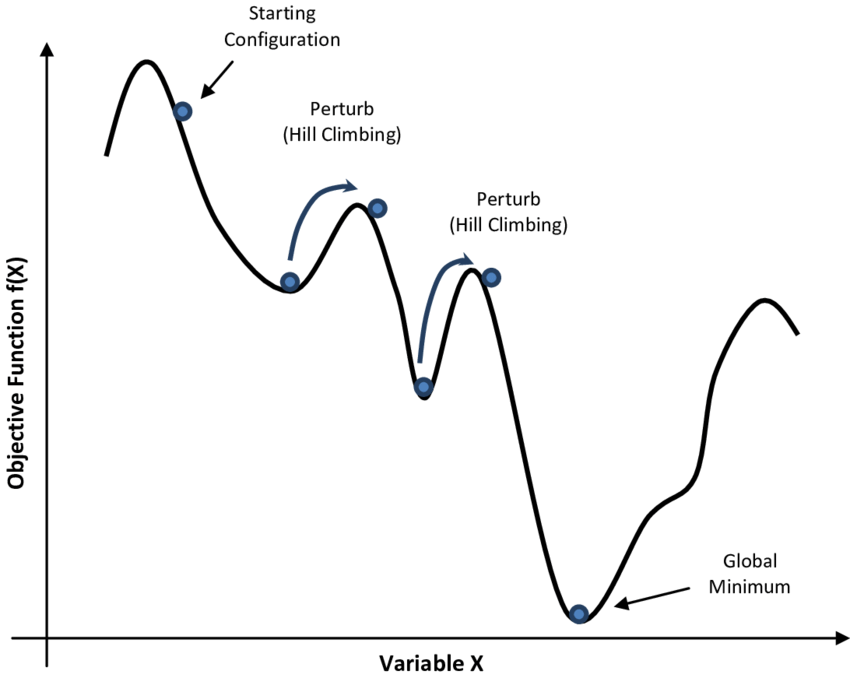
\includegraphics[height=0.5\textheight]{images/SimulatedAnnealingIllustration.png}\footnote[frame]{https://www.researchgate.net/figure/Simulated-Annealing-optimization-of-a-one-dimensional-objective-function\_fig1\_308786233}}
				\only<7>{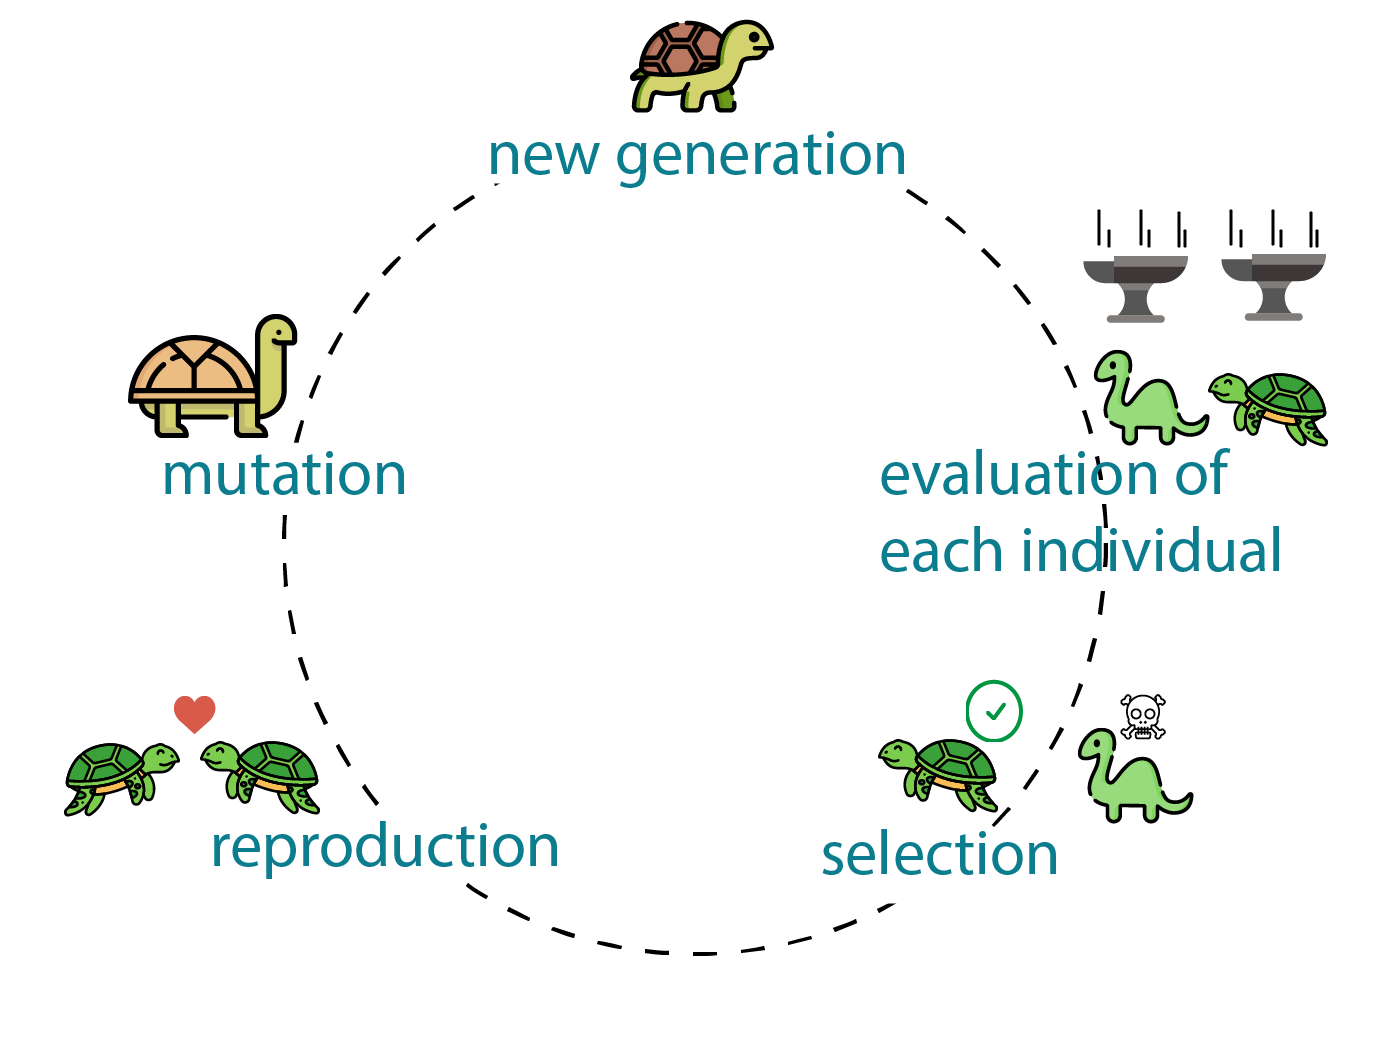
\includegraphics[height=0.5\textheight]{images/geneticAlgorithmIllustration'.png}\footnote[frame]{https://www.generativedesign.org/02-deeper-dive/02-04\_genetic-algorithms/02-04-01\_what-is-a-genetic-algorithm}}
				\only<12->{
				\begin{block}{UI extensions: more paramteters, different interface}
					\only<12-16>{
					\begin{itemize}
						\item<13-> Using previously mentioned attributes
						\item<14-> In the implementation and UI
						\item<15-> Change UI appearance accordingly
					\end{itemize}}
				\only<17>{
					\begin{itemize}
						\item Using previously mentioned attributes \checkmark
						\item In the implementation and UI 
						\item Change UI appearance accordingly
					\end{itemize}}
				\only<18>{
					\begin{itemize}
						\item Using previously mentioned attributes \checkmark
						\item In the implementation and UI \textbigcircle
						\item Change UI appearance accordingly
					\end{itemize}}
				\only<19->{
					\begin{itemize}
						\item Using previously mentioned attributes \checkmark
						\item In the implementation and UI \textbigcircle
						\item Change UI appearance accordingly \checkmark
					\end{itemize}}
				\end{block}
			\textcolor{white}{a}\\
			\textcolor{white}{a}}
			\end{minipage}}
		\only<20->{$\Rightarrow$ Generally: change Tour4Me so that it can generate and show a (as good as possible) solution for (almost) every starting point and configuration}
	\end{frame}
	
	\begin{frame}
	\vspace{0.25cm}
	What are the goals? What did I do so far?

	\vspace{0.25cm}
	\centering
	\only<1>{\includegraphics[height=0.8\textheight]{images/fullAppAll_hidden.png}}
	\only<2>{\includegraphics[height=0.8\textheight]{images/fullApp_options_open.png}}
	\only<3>{\includegraphics[height=0.8\textheight]{images/options_algorithm_select.png}}
	\only<4>{\includegraphics[height=0.8\textheight]{images/ant_tour.png}}
	\only<5>{\includegraphics[height=0.8\textheight]{images/ant_tour_high_importance_covered_area.png}}
	\only<6>{\includegraphics[height=0.8\textheight]{images/ant_result.png}}
	\only<7>{\includegraphics[height=0.8\textheight]{images/min_vs_antMin.png}}
	\only<8>{\includegraphics[height=0.8\textheight]{images/greedy_vs_antGreedy.png}}
	\only<9>{\includegraphics[height=0.8\textheight]{images/greedy_vs_simulatedAnnealing.png}}
	\only<10>{\includegraphics[height=0.8\textheight]{images/simulatedAnnealing_stats.png}}
	\only<11->{
		\begin{block}{Database}
			\pause	
			\only<11->{
				\pause
				\begin{itemize}
					\item<12-> DB import script for other cities than Dortmund
					\item<13->  Adding elevation data
					\item<14->  Adding surroundings data
					\item<15->  Building a spatial DB $\rightarrow$ getting subgraphs is easier
			\end{itemize}}
		\end{block}}
	\only<16->{
		\begin{block}{Parameter testing visualization}
			\pause	
			\only<16->{
				\pause
				\begin{itemize}
					\item<17-> Graph visualization (all edges) $\rightarrow$ removing dead ends, checking undesirable path removal
					\item<18-> Script for visualizing different result paths with varying parameters (so far only for a few ant colony parameters)
			\end{itemize}}
		\end{block}}
	\end{frame}
	
	
%	\section{Literatur}
%	\begin{frame}[allowframebreaks]{Literatur}
%		
%		\bibliography{LS11Buchin.bib}
%	\end{frame}
%	
	
\end{document}

